\documentclass{article}
\usepackage{graphicx}
\usepackage[a4paper, total={16cm, 24cm}]{geometry}
\usepackage{xspace}
\usepackage[hidelinks]{hyperref}
\usepackage{color}
\usepackage{fancyvrb}
\newcommand{\shiv}{\texttt{shiver}\xspace}
\newcommand{\sac}{\texttt{shiver\char`_align\char`_contigs.sh}}
\let\c\texttt
\newcommand{\www}{\color{blue} \underline}

\title{\shiv\\available from \href{https://github.com/ChrisHIV/shiver}{\www{https://github.com/ChrisHIV/shiver}}}
\date{This manual last updated \today}
\author{By Chris Wymant}

\begin{document}
\maketitle


\begin{figure}[!h]
\centering
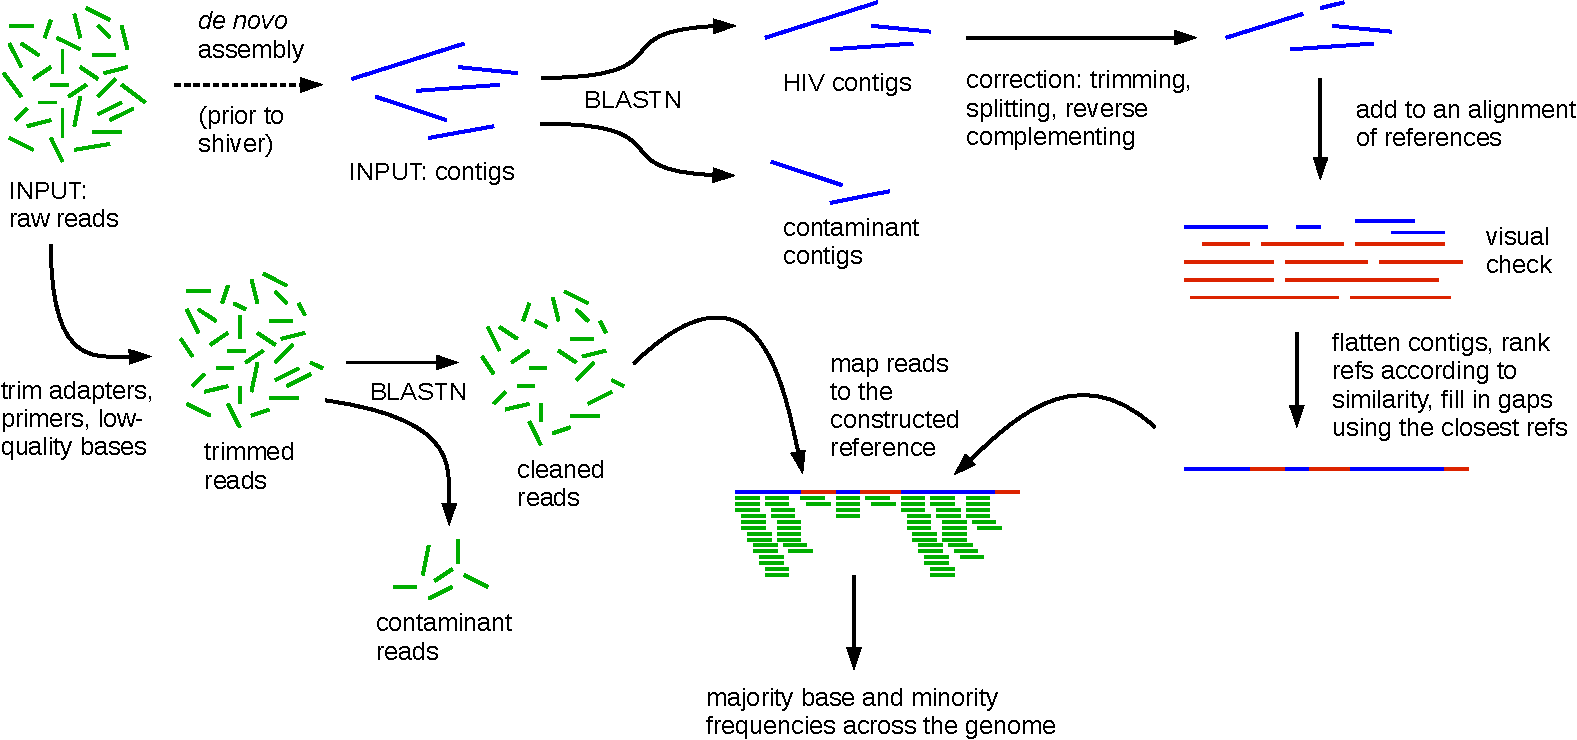
\includegraphics[width=0.95\textwidth]{AssemblyPipelineDiagram_ForPaper.pdf}
\end{figure}


\shiv is a tool for mapping paired-end short reads to a custom reference sequence constructed using do novo assembled contigs, in order to minimise the biased loss of information that occurs from mapping to an reference that differs from the sample.
From the mapped reads, base frequencies are quantified, and a consensus sequence is called.
\shiv was designed for HIV but has broader applicabilty; if you are using it for sequence data from organism X instead of HIV, mentally replace {\it HIV} by {\it X} when reading this manual.

The method and its performance are discussed in \cite{Wymant092916}; please cite this if you find \shiv helpful.
If you use \shiv, please also cite the publications of its dependencies: \c{SAMtools}~\cite{Li08062009}, \c{MAFFT}~\cite{Katoh15072002}, \c{trimmomatic}\cite{Bolger01082014}, \c{BLAST}~\cite{ALTSCHUL1990403}, and \c{BWA}~\cite{doi:10.1093/bioinformatics/btp698} or \c{bowtie}~\cite{Langmead2009} if you switched the default mapper from \c{smalt} (for which there is no publication to cite).
Details of these are found in the file \c{CitationDetails.bib} in \shiv's \c{info} subdirectory.

If you have a problem getting the code to run or think you've found a bug, please create a \href{https://github.com/ChrisHIV/shiver/issues}{\www{\it New issue}} on the GitHub repository.

Throughout this manual, I'll assume your \shiv code lives in \c{\path{~}/shiver/}.
If you downloaded it somewhere else, e.g. \c{my/other/directory/shiver/}, simply replace every occurence of \c{\path{~}/shiver/} in by \c{my/other/directory/shiver/} (or if you're feeling lazy, create a link to \c{my/other/directory/shiver}, call it \c{shiver}, and put it in your home directory).

By default, to run \shiv commands, you have to tell the command line where those commands can be found, i.e. include their path: \c{\path{~}/shiver/shiver\char`_align\char`_contigs.sh}.
If you don't want to type the path every time, so that you can just type \sac, you need to add the directory containing the \shiv code (\c{\path{~}/shiver/}) to your \c{PATH} environmental variable.
Google this if you don't know how to do that.

Throughout this manual, a \c{\$} character at the start of a line just indicates that what follows should be run from command line -- it should not be entered as part of your command.


\section{Initialisation}
Before you begin processing a collection of samples there's an initialisation step: it should be run once only (i.e. not once for each sample).
It requires  
\begin{itemize}
\item The \shiv configuration file, named by default \c{config.sh}.
(Here it is needed only to tell \shiv how to run the program blast; you can change your mind about all the pipeline parameters contained in this file later on. See also the section {\it The config file}.);  
\item An alignment of your choice of existing reference genomes (lots of which are available to download from the \href{http://www.hiv.lanl.gov/content/sequence/NEWALIGN/align.html}{\www{Los Alamos National Lab}}) called \c{RefAlignment.fasta}, say.  
\item Fasta files containing the adapters and primers used for sequencing, called \c{adapters.fasta} and \c{primers.fasta}, say.
(Adapters will be removed using trimmomatic, and ``The naming of the various sequences within this file determines how they are used'' -- trimmomatic docs.
In the \c{ExampleInput} directory of this repository is a default Illumina adapters file, and a file containing the primers relevant to our sequence data -- those of Gall {\it et al.} (J. Clin. Microbio. 2012).
{\bf Do not} assume these are what's needed for your sequence data -- instead ask your sequencing team to provide the adapter and primer sequences they used.)
\end{itemize}


Initialisation files will be put into a directory called \c{MyInitDir} if you run
\begin{Verbatim}[samepage=true]
$ ~/shiver/shiver_init.sh  MyInitDir  config.sh  RefAlignment.fasta  adapters.fasta \
  primers.fasta
\end{Verbatim}
(remembering to skip that first \c{\$} character.)
You shouldn't touch \c{MyInitDir} or the files therein after running this command, or unknown bad things might happen.

After running that initialisation command (once only!) you can process any number of samples.
Since sample processing generates (many) files in the working directory, to avoid overwriting files you should always work in an empty directory for each sample, as illustrated in the {\it Scripted usage to process batches of samples} section below.

\section{\shiv input}
The input for each sample is (1) paired-end short reads, and (2) contigs generated by running {\it de novo} assembly on those short reads.
\begin{enumerate}
\item The forward read names must all end in ``/1'', the reverse read names must all end in ``/2'', and mates in a pair must match in what comes before this.
e.g. Forward read names might be {\it FirstReadName/1}, {\it SecondReadName/1}, $\ldots$ and reverse read names should then be {\it FirstReadName/2}, {\it SecondReadName/2}, $\ldots$ This is so \shiv knows how to pair the reads together.
\item Our chosen assembler is IVA; it can be installed from \href{http://sanger-pathogens.github.io/iva/}{\www{here}} or run on a virtual machine \href{http://sanger-pathogens.github.io/pathogens-vm/}{\www{here}}, and the publication is \href{http://bioinformatics.oxfordjournals.org/content/early/2015/02/27/bioinformatics.btv120.abstract}{\www{here}}.
Say your forward reads are in \c{reads\char`_1.fastq.gz} and your reverse reads are in \c{reads\char`_2.fastq.gz}; assembling them into contigs is as simple as running
\begin{Verbatim}[samepage=true]
$ iva  -f  reads_1.fastq.gz  -r  reads_2.fastq.gz  MyOutputDirectory
\end{Verbatim}
though you should run \c{iva --help} to see the options, including specifying adapter and primer sequences to trim from the reads.
\shiv wants {\it all} contigs produced by assembly; if by curiosity you check what organisms the different contigs come from, do not remove non-HIV contigs.
These contaminant contigs (if present) are used to help remove contaminant reads.

\end{enumerate}


\section{How to process a single sample}
Processing requires two commands.
With forward/reverse read files named as above and contigs in \c{contigs.fasta}, the first is  
\begin{Verbatim}[samepage=true]
$ ~/shiver/shiver_align_contigs.sh  MyInitDir  config.sh  contigs.fasta  SID
\end{Verbatim}
replacing \c{SID} (`sample ID') by a name used for labelling all output files for this sample.
This command will produce a file named \c{SID.blast} (detailing blast hits of your contigs to those existing references supplied for the initialisation).
Assuming at least one contig looks like HIV, \c{SID.blast} will not be empty (see section {\it Including samples without contigs} otherwise), and there will be another file called \c{SID\char`_raw\char`_wRefs.fasta} -- an alignment of the HIV contigs (i.e. those that have blast hits) to your input existing reference genomes.
As discussed in the \shiv article, this alignment should be inspected, and in the minority of cases where this is required, edited; see the following section.

\shiv decides that a contig needs correcting, if it
\begin{itemize}
 \item is not wholly spanned by a blast hit, suggesting that the ends are not genuine HIV and should be trimmed off;
 \item has two or more blast hits (ignoring hits wholly inside other hits), suggesting that it is chimeric/spliced -- erroneously connecting disconnected parts of the genome;
 \item has a blast hit in the opposite orientation to the reference, suggesting that that contig (or part of the contig) should be reverse complemented;
 \item contains an unrealistically large gap after alignment, to the existing references, suggesting that it should be split into two separate contigs.
\end{itemize}
Appropriate action is taken in each case, cutting and reverse-complementing as needed.
If any of these actions were needed for any of the contigs, an additional file \c{SID\char`_cut\char`_wRefs.fasta} will be produced, which contains all contigs after correction aligned to the existing references.
We expect that \c{SID\char`_cut\char`_wRefs.fasta} (if it exists) is a better alignment than \c{SID\char`_raw\char`_wRefs.fasta}, but it's safer not to take this for granted, for example unusual indels can result in multiple blast hits.
It's therefore recommended to inspect both alignments, choose which set of contigs you think are more likely to approximate the true consensus, edit the alignment if you spot what you believe to be errors, and discard the other alignment. 

With an alignment of contigs you're happy with, say \c{SID\char`_raw\char`_wRefs.fasta}, run
\begin{Verbatim}[samepage=true]
$ ~/shiver/shiver_map_reads.sh  MyInitDir  config.sh  contigs.fasta  SID  \
  SID.blast  SID_raw_wRefs.fasta  reads_1.fastq.gz  reads_2.fastq.gz
\end{Verbatim}
and you're done.
You'll probably want to delete the intermediate files produced during processing (beginning with \c{temp} by default), i.e. \c{rm temp*}.

\section{A manual step between the two automatic steps? Blasphemy!}
The reason for this is discussed in more detail in the \shiv paper.
Correct alignment has already been attempted automatically in the first step, but unfortunately aligning whole HIV genomes automatically, perfectly, 100\% of the time is a dream: HIV has very high mutation and substitution rates, including frequent insertions and deletions.
Compounding this problem is the fact that de novo assembly output is sometimes an imperfect representation of the sample, and aligning problematic sequences may give problematic alignments. 
For most samples the contigs and their alignment are fine, and seeing this from the alignment takes one or two seconds of human time.
When editing is required, it amounts to one of two things: deleting a whole contig if it appears to be wholly junk (i.e. short stretches of poorly aligned sequence separated by large gaps), or deleting the end of a contig if just the end looks wrong (i.e. a stretch of sequence in very poor agreement with the existing references, or a stretch of sequence separated from the rest of the contig by a gap implausibly large for a real deletion).
Visually checking and editing when needed ensures an alignment of contigs you can trust, allowing the second \shiv command to reliably construct a) a tailored reference that minimises mapping bias, and b) a global alignment of all samples, instantly, without further need for an alignment algorithm: see the end of section {\it Scripted usage to process batches of samples}.  
\href{https://github.com/olli0601/PANGEAhaircut}{\www{This}} R package by Oliver Ratmann uses machine learning to correct such alignments; however for each sample you must manually check the corrections to ensure they are correct, instead of checking the alignment itself.

\section{What output do I get?}
\begin{itemize}
\item \c{SID.bam}, \c{SID\char`_ref.fasta}: the bam file of mapped reads, and the reference to which they were mapped.
(It's a shame the bam file format does not include the reference, c'est la vie.)
\item \c{SID\char`_BaseFreqs.csv}: the frequencies of A, C, G, T, `-' for a deletion, and N for unknown, at each position in the genome.
\c{SID\char`_BaseFreqs\char`_ForGlobalAln.csv} is almost the same thing; it contains an extra column with a coordinate that can be used to compare different samples, at the cost of having to skip some rows for which the coordinate is not defined (see section~\ref{sec:GlobalAln}).
\c{SID\char`_BaseFreqs\char`_WithHXB2.csv} contains the base frequencies and an extra column for the coordinate in HXB2; again this has the cost of needing to exclude some rows (where the reads had an insertion with respect to the reference).
\item \c{SID\char`_MinCov\char`_X\char`_Y.fasta}: the pairwise alignment of the consensus genome and the reference used for mapping.
In place of \c{X} and \c{Y} here you'll see the two coverage thresholds specified in \c{config.sh}: \c{X} is the minimum number of reads to call a base (if there are fewer than \c{X} reads we call \c{?} instead of a base), \c{Y} the minimum number to use upper case for the base (to signal increased confidence).
The mapping reference is included with the consensus here to give context to any \c{?} characters.
\item \c{SID\char`_MinCov\char`_X\char`_Y\char`_ForGlobalAln.fasta}, \c{SID\char`_coords.csv}: these files are useful for when multiple samples are processed, so we postpone their explanation to section~\ref{sec:GlobalAln}.  
\item \c{SID\char`_clean\char`_1.fastq}, \c{SID\char`_clean\char`_2.fastq}: the unmapped reads after removal of adapters, primers, low-quality bases, and those read pairs suspected of being contamination.  
\item \c{SID\char`_InsertSizeCounts.csv}: the insert-size distribution.
\end{itemize}


Files that are not produced by default, but whose production can be specified in \c{config.sh}:
\begin{itemize}
\item \c{SID\char`_MinCov\char`_X\char`_Y\char`_wContigs.fasta}: an alignment of the consensus, the reference used for mapping, and all HIV contigs for this sample (as they were after any automatic cutting and any manual editing).
\item \c{SID\char`_ContaminantReads.bam}: a bam file of only the contaminant reads mapped to the HIV reference (to illustrate the importance of removing these reads from the HIV reads prior to mapping).
\end{itemize}

If the config file variable \c{remap} is left at its default value of \c{true}, some of the files named above will have a second copy with \c{SID} replaced by \c{SID\char`_remap} in the file name: these will likely be very similar, but expected to be slightly more accurate -- if they exist, use them instead.

\section{The config file}
In \c{config.sh} you can change pipeline parameters from their default values.
During development of \shiv, \c{config.sh} has often been updated (e.g. new features might require new parameters).
As this may happen again in the future, to make sure you keep any changes you've made to default values, I recommend the following: make one copy of \c{config.sh} called \c{config\char`_original.sh}, a second copy called \c{config\char`_MyChanges.sh}, leave the former untouched and change whatever you like in the latter.
Then when you update your \shiv code, running
\begin{Verbatim}[samepage=true]
$ diff config_original.sh ~/shiver/config.sh
\end{Verbatim}
will show you whether the update has changed the config file; if so, running
\begin{Verbatim}[samepage=true]
$ diff config_original.sh config_MyChanges.sh
\end{Verbatim}
will remind you of the changes you made to default parameter values.


\section{Scripted usage to process batches of samples}
Before we start, note that scripted use of \shiv (like any other command-line program) to process multiple files is easier if you know the basics of playing with filenames from the command line.
Consider this toy example:
\begin{Verbatim}[samepage=true]
# We have two directories: one with text files, one with csv files.
$ ls CsvDir/
bar.csv  foo.csv
$ ls TxtDir/
bar.txt  foo.txt
# Assign the text file we want to a variable:
$ DesiredTextFile=TxtDir/foo.txt
# This shows how to find the associated csv file:
$ DesiredTextFileNoPath=$(basename "$DesiredTextFile")
$ echo "$DesiredTextFileNoPath"
foo.txt
$ DesiredTextFileNoPathNoExtention="${DesiredTextFileNoPath%.txt}"
$ echo "$DesiredTextFileNoPathNoExtention"
foo
$ AssociatedCsvFile=CsvDir/"$DesiredTextFileNoPathNoExtention".csv
$ ls "$AssociatedCsvFile"
CsvDir/foo.csv
# Or, the above steps all in one go:
$ DesiredTextFile=TxtDir/foo.txt
$ ls CsvDir/$(basename "${DesiredTextFile%.txt}").csv
CsvDir/foo.csv
\end{Verbatim}

Now back to \shiv.
Say your current directory contains three subdirectories: \c{contigs}, \c{MyInitDir} and \c{reads}, containing what the name suggests.
Here are your contigs:
\begin{Verbatim}[samepage=true]
$ ls contigs/
sampleA.fasta sampleB.fasta sampleC.fasta
\end{Verbatim}
and here are your reads:
\begin{Verbatim}[samepage=true]
$ ls reads/
sampleA_1_fastq.gz sampleA_2_fastq.gz  
sampleB_1_fastq.gz sampleB_2_fastq.gz  
sampleC_1_fastq.gz sampleC_2_fastq.gz
\end{Verbatim}
Start by aligning the contigs for all samples:
\begin{Verbatim}[samepage=true]
$ for ContigFile in contigs/*.fasta; do  
  # Extract the SID from the filename: remove the extension and the path
  SID=$(basename "${ConfigFile%.fasta}")
  # Make, and change into, an empty directory for processing this contig file
  mkdir AlignmentOutput_"$SID"  
  cd AlignmentOutput_"$SID"  
  ~/shiver/shiver_align_contigs.sh ../MyInitDir ../config.sh "$ContigFile" "$SID"
  cd ..
done
\end{Verbatim}
As explained above, for those samples for which contig correction is necessary, \c{SID\char`_cut\char`_wRefs.fasta} will be produced as well as \c{SID\char`_raw\char`_wRefs.fasta}, and only the better looking of these two should be kept (and edited if needed).
Let's say you put one of these two files for each sample all together in a directory called \c{CheckedContigAlignments}.  
\begin{Verbatim}[samepage=true]
# For samples that had an SID_cut_wRefs.fasta file, we kept either that file or
# SID_raw_wRefs.fasta. Let's rename all these files to have the same suffix -
# removing '_raw' or '_cut' to leave just SID_wRefs.fasta - to make it easier
# to find the one we want.  
$ cd CheckedContigAlignments  
$ for alignment in *_cut_wRefs.fasta; do
  mv -i "$alignment" "${alignment%_cut_wRefs.fasta}"_wRefs.fasta
done
$ for alignment in *_raw_wRefs.fasta; do
  mv -i "$alignment" "${alignment%_raw_wRefs.fasta}"_wRefs.fasta
done
# Now let's map! Make and change into an empty directory for processing each sample.
$ cd ..
$ for ContigFile in contigs/*.fasta; do  
  # Find the other files for this sample.
  # NB careful scripting would check that files exist before using them.
  SID=$(basename "${ConfigFile%.fasta}")
  mkdir MappingOutput_"$SID"
  cd MappingOutput_"$SID"
  BlastFile=../AlignmentOutput_"$SID"/"$SID".blast
  alignment=../CheckedContigAlignments/"$SID"_wRefs.fasta
  reads1=../reads/"$SID"_1.fastq.gz
  reads2=../reads/"$SID"_2.fastq.gz
  ~/shiver/shiver_map_reads.sh ../MyInitDir ../config.sh "$ContigFile" \
  "$SID" "$BlastFile" "$alignment" "$reads1" "$reads2"
  cd
done
\end{Verbatim}
and you're done mapping.

\section{The Global Alignment} \label{sec:GlobalAln}

Now for those aforementioned \c{*\char`_MinCov\char`_X\char`_Y\char`_ForGlobalAln.fasta} files.
These are generated by excising unique insertions seen in a sample (i.e. not seen in any of the existing references used for initialisation), and then inserting gaps using coordinate translation in such a way that these files are all aligned with each other and with the alignment of existing references.
Constructing a global alignment is then achieved just by putting all those files into one file:
\begin{Verbatim}[samepage=true]
$ cat MappingOutput_*/*_ForGlobalAln.fasta > GlobalAln.fasta
$ cat MyInitDir/ExistingRefAlignment.fasta >> GlobalAln.fasta
\end{Verbatim}
Now it's over to you for phylogenetics, GWAS etc.

\section{Including samples without contigs}
You might have some samples for which none of the contigs have blast hits to the existing references you supplied, i.e. it looks like all contigs are contaminants.
In this case the contig alignment step will produce an empty blast file and no \c{SID\char`_raw\char`_wRefs.fasta} file.
If you have total confidence in your {\it de novo} assembler, you could choose to dismiss such samples as total sequencing failure -- that would be reasonable.
On the other hand perhaps there are enough HIV reads to call a partial consensus, and the assembler just failed to build any contigs out of them.
Because of this possibility, in place of the alignment-of-contigs-to-existing-references argument that's given to \c{shiver\char`_map\char`_reads.sh}, you can supply a fasta file containing a single sequence: that sequence will be used as the reference for mapping, instead of a tailored one constructed from contigs.
If that sequence is one of the existing references you provided at the initialisation step, \shiv knows how to do the coordinate translation necessary to produce a \c{SID\char`_MinCov\char`_X\char`_Y\char`_ForGlobalAln.fasta} file; if not, this file will not be produced (you'll still get your consensus sequence though).

To script this kind of thing, you can just check whether the alignment of contigs to existing references exists for this sample: if not, choose a sequence to use as your reference to mapping.
This would probably be most easily achieved by making a big look-up table before you start.
(e.g. running the program \href{https://ccb.jhu.edu/software/kraken/}{\www{kraken}} or \href{https://pachterlab.github.io/kallisto/}{\www{kallisto}} on the reads for each sample, one can see which of the existing references has the largest number of reads attributed to it; one might obtain a non-null result even when no HIV contigs were assembled.)
For example in the scripted usage above, after \\\c{alignment=../CheckedContigAlignments/"\$SID"\char`_wRefs.fasta}, you could have
\begin{Verbatim}[samepage=true]
  if [[ ! -f "$alignment" ]]; then
    # Reassign the $alignment variable to be a file containing
    # the reference previously chosen for this sample.
  fi
\end{Verbatim}

\section{Sample Reprocessing and Analysis}
Individual steps from \shiv can be run with stand-alone command line tools, for ease of reapplication elsewhere; these are contained in the \c{tools} subdirectory of the \shiv code directory.
For example \texttt{CorrectContigs.py} is run with a file of contigs and a file of their \texttt{BLASTN} hits to some set of references, and corrects the contigs by cutting and reverse-complementing where needed.
%, such as \texttt{AnalysePileup.py} which parses pileup format into simple base frequencies, \texttt{ConstructBestRef.py} which constructs the trailored reference by flattening contigs and filling in gaps with the closest references to those contigs, and 
Also included in \shiv are command-line tools for easy analysis and modification of sample output without rerunning the whole pipeline:
\begin{itemize}

\item Recall \c{X} and \c{Y} above -- the coverage thresholds for calling bases.
You can generate another consensus sequence using different values, \c{X2} and \c{Y2} say, without rerunning the whole pipeline, thus:
\begin{Verbatim}[samepage=true]
$ tools/CallConsensus.py SID_BaseFreqs.csv X2 Y2 > MyNewConsensus.fasta
\end{Verbatim}
If you decrease the value of \c{X} you will see more bases and fewer \c{?} characters: the less strict you are with your requirement on `vertical' coverage (the number of mapped bases at a point; the height at a given position in the bam file, if you like), the more `horizontal' coverage (i.e. genomic coverage, the total number of bases called in the consensus) will increase.
That's good right?
Yes and no.
You could also increase your horizontal coverage by replacing all ? characters by a random selection of As, Cs, Gs and Ts, but it's not recommended.
Decreasing these thresholds increases sensitivity to HIV reads at the cost of specificity (since some reads are bound to be contaminants), and you ought to balance these, not just maximimise the former.
For example with dated sequences, you could try to get the strongest correlation between real time and the evolutionary distance inferred from a phylogeny -- the $R^2$ of the molecular clock -- since too little real sequence and too much contaminant sequence will both screw up your phylogeny.
To regenerate a coordinate-translated version of this consensus for the global alignnent (of all consensuses produced by shiver), \c{tools/TranslateSeqForGlobalAln.py} can be run, taking as its two arguments the consensus, and \c{SID\char`_coords.csv} generated by the full run of shiver.

\item Another parameter in the configuration file is the minimum read {\it identity} -- the fraction of bases in the read which are mapped and agree with the reference -- required for a read to be considered mapped, and so retained in the BAM file.
If you wish to increase this after completion of \shiv, reads with an identity below your new higher threshold can be discarded by running \texttt{RemoveDivergentReads.py} on a BAM file.
Running \texttt{shiver\char`_reprocess\char`_bam.sh} on the resulting BAM file (or indeed any BAM file) implements just the last steps in \shiv, namely generating pileup, calculating the base frequencies, and calling the consensus.

\item \texttt{FindNumMappedBases.py} calculates the total number of mapped bases in a BAM file (where read length is constant this equals the number of mapped reads multiplied by read length, minus the total length of sequence clipped from reads), optionally binned by read identity.
In the absence of mapped contaminant reads, and all else being equal, mapping to a reference which is closer to the true consensus should map more bases and mapped reads should have higher identities.
%It was used to produce Fig.~\ref{fig:NumMappedBases}.

\item \texttt{FindClippingHotSpots.py} counts, at each position in the genome, the number and percentage of reads that are clipped from that position to their left or right end.
Having many such reads is a warning sign of the kind of biased loss of information discussed in the \shiv paper.

\item \texttt{FindSubSeqsInAlignment.py} finds the location of specified subsequences in an alignment.

\item \texttt{LinkIdentityToCoverage.py} finds, for each different coverage encountered when considering all positions in a BAM file, the mean read identity at such positions.
The mean read identity tends to be lower at positions of low coverage due to a background of contaminant reads, which differ from the reference by virtue of being contamination, but which are nevertheless similar enough to be mapped.
Quantifying the decline in identity at low coverage helps inform what coverage threshold is appropriate for a given data set.

\item \texttt{AlignMoreSeqsToPairWithMissingCoverage.py} allows more sequences to be added to a pairwise alignment in which one sequence contains missing coverage (such as a consensus and its reference), correctly maintaining the distinction between gaps (indicating a deletion) and missing coverage.

\item \texttt{AlignBaseFreqFiles.py} aligns not two sequences, but two of the csv-format base frequency files output by \shiv.
Optionally a similarity metric is calculated at each position in the alignment, between 0 (no agreement on which bases/gaps are present) and 1 (perfect agreement on which bases/gaps are present and on their proportions).
This allows comparison not just of consensus sequences between two samples but also of minority variants.

\item \texttt{ConvertAlnToColourCodes.py} converts each base in a sequence alignment into a colour code indicating agreement with the consensus and indels; \texttt{AlignmentPlotting.R} takes such colour codes and visualises the alignment.
These scripts were used to produce the alignment + coverage + gene diagrams in the \shiv paper.

\item Finally some simple tools for convenience: \texttt{FindSeqsInFasta.py} extracts named sequences from a fasta file, with options including gap stripping, returning only windows of the sequences, and inverting the search; \texttt{PrintSeqLengths.py} prints sequence lengths with or without gaps; \texttt{SplitFasta.py} splits a fasta file into one file per sequence therein.
\end{itemize}


\bibliographystyle{ieeetr}
\bibliography{CitationDetails}

\end{document}